\documentclass[11pt]{article}
\usepackage[T1]{fontenc}
\usepackage{lmodern}
\pdfglyphtounicode{parenleftbig}{0028}
\pdfglyphtounicode{parenrightbig}{0029}
\pdfglyphtounicode{parenleftBig}{0028}
\pdfglyphtounicode{parenrightBig}{0029}
\pdfgentounicode=1
\usepackage[margin=1.05in]{geometry}
\usepackage{amsmath,amssymb,amsthm,mathtools}
\usepackage{microtype}
\usepackage{enumitem}
\usepackage{tikz}
\usetikzlibrary{arrows.meta,positioning,calc}
\usepackage[hidelinks]{hyperref}
\hypersetup{pdftitle={A proof of Seymour's second-neighborhood conjecture},
 pdfauthor={OpenAI}, pdfsubject={Oriented graphs and finite relations}}
\pdftrailerid{}
\newtheorem{theorem}{Theorem}[section]
\newtheorem{lemma}[theorem]{Lemma}
\newtheorem{proposition}[theorem]{Proposition}
\newtheorem{corollary}[theorem]{Corollary}
\theoremstyle{remark}
\newtheorem{remark}[theorem]{Remark}
\newcommand{\abs}[1]{\lvert #1\rvert}
\DeclareMathOperator{\rank}{rank}
\DeclareMathOperator{\im}{im}
\newcommand{\R}{\mathbb R}
\newcommand{\unverified}[1]{\par\smallskip\noindent\fbox{\parbox{0.95\linewidth}{\textbf{Unverified step.} #1}}\par\smallskip}
\newcommand{\step}[1]{\par\medskip\noindent\textbf{#1}\enspace}
\newcommand{\TT}{\mathrm{TT}}
\title{A proof of Seymour's second-neighborhood conjecture}
\author{Rewritten for readability from the OpenAI manuscript of the same title}
\date{September 23, 2026}
\begin{document}
\maketitle
\begin{abstract}
We prove that every nonempty finite oriented graph has a vertex with at least
as many vertices at directed distance two as at directed distance one.
This resolves Seymour's second neighborhood conjecture positively.
This version is a step-by-step rewrite of the source manuscript with the same
statements and the same proof strategy.  One sentence of the source (Step~1 in
the proof of Lemma~\ref{lem:subset-deficit}) is false as written; it is kept
and flagged in a box, together with the one-word change that makes it correct.
\end{abstract}

\section{The result and the plan}\label{sec:introduction}

\subsection{Statement}

An \emph{oriented graph} is a finite directed graph with no loops, no multiple
arcs, and no pair of opposite arcs.  Its underlying undirected graph need
not be complete or connected.  We write $v\to u$ when there is an arc from $v$
to $u$.  For a vertex \(v\), put
\[
 N_1^+(v)=\{u:v\to u\},\qquad
 N_2^+(v)=\{w\notin\{v\}\cup N_1^+(v):
                 \text{ there is a vertex }u\text{ with }v\to u\to w\}.
\]
Thus \(N_2^+(v)\) consists of the vertices at directed distance exactly two
from \(v\); each is counted once, however many paths reach it.

\begin{theorem}\label{thm:main}
Every nonempty finite oriented graph has a vertex \(v\) such that
\[
 \abs{N_1^+(v)}\leq \abs{N_2^+(v)}.
\]
\end{theorem}

This is Seymour's second neighborhood conjecture.  No connectivity or degree
hypothesis is needed.

\emph{Sanity checks.}  A sink (a vertex with no out-neighbor) satisfies the
conclusion, as $0\le 0$.  In a directed triangle every vertex has
$\abs{N_1^+}=\abs{N_2^+}=1$.  In the transitive triangle $a\to b\to c$,
$a\to c$, the vertex $a$ has $N_1^+(a)=\{b,c\}$ and $N_2^+(a)=\varnothing$,
because $c$ is already reached in one step.  So removing first out-neighbors
from $N_2^+$ is essential to the assertion, and here only the sink $c$ works.

\subsection{Notation used throughout}\label{subsec:notation}

For a digraph \(D\) and a set \(S\subseteq V(D)\), the \emph{image} of $S$ is
\[
 F_D(S)=\{y:\text{ there is }x\in S\text{ with }x\to y\},
 \qquad F_D^2(S)=F_D(F_D(S)).
\]
The operator \(F_D\) does \emph{not} subtract \(S\), so $F_D(S)$ may meet $S$.
We use three elementary facts.
\begin{enumerate}[label=\textup{(F\arabic*)},leftmargin=3em]
\item\label{F1} $F_D(\varnothing)=\varnothing$,
 $F_D(A\cup B)=F_D(A)\cup F_D(B)$, and $A\subseteq B$ implies
 $F_D(A)\subseteq F_D(B)$.
\item\label{F2} If $D$ is oriented, then $N_1^+(v)=F_D(\{v\})$ and
 $N_2^+(v)=F_D^2(\{v\})\setminus F_D(\{v\})$.
 Indeed, $F_D^2(\{v\})$ is the set of ends $w$ of walks $v\to u\to w$.
 Such a walk never has $w=v$, since $v\to u\to v$ would be a pair of
 opposite arcs.  So removing $N_1^+(v)$ leaves exactly $N_2^+(v)$.
\item\label{F3} Every vertex of $D$ has positive indegree if and only if
 $F_D(V(D))=V(D)$.
\end{enumerate}
When two graphs are in play we write $N^+_{1,D}$, $N^+_{2,D}$ to indicate
the graph.

\emph{Renamed symbols.}  To keep one meaning per letter, a few symbols of the
source are renamed, as follows.
\begin{itemize}[nosep]
\item In Lemma~\ref{lem:subset-deficit}, the set of lost out-neighbors is $Y$
 (source: $Q$).
\item In Lemma~\ref{lem:blowup}, label sets are $\Lambda,\Lambda_v$
 (source: $T,T_v$), and the transitive tournament is $\TT_m$ (source: $T_m$).
\item In Section~\ref{sec:pruning}, the support-rank matrices are
 $\Phi,\Phi^{p,i}$ with supports $\Sigma,\Sigma^{p,i}$ (source: $D,D^{p,i}$,
 $T,T^{p,i}$).  The index sets of Lemma~\ref{lem:kernel-support} are
 $\mathcal I,\mathcal J$ (source: $I,J$), and its vectors are bold
 $\mathbf x,\mathbf y,\mathbf h$ (source: $x,y,w$).
\item In Section~\ref{sec:weighted-consequences}, the arc weighting is $\omega$
 and the associated quantity is $\kappa^\omega_v$ (source: $w$, $\beta_v^w$);
 the matrix is $\mathsf M_D$ (source: $M_D$).
\item In Section~\ref{sec:directed-cycle-consequences}, the non-neighbor set is
 $N^0(v)$ (source: $Z(v)$).
\end{itemize}
Sections~\ref{sec:weighted-consequences}
and~\ref{sec:directed-cycle-consequences} come after the proof of
Theorem~\ref{thm:main} and use a few letters locally.

\subsection{Proof at a glance}\label{subsec:glance}

The proof is by contradiction and has three parts.  Parts A and B are
independent of each other; Part C uses Part B, and the theorem follows from
A and C.

\paragraph{Part A (Section~\ref{sec:reduction},
Proposition~\ref{prop:counterexample-reduction}).}
If a counterexample exists, then there is an oriented graph $G$ with all
indegrees positive such that
\begin{equation}\label{eq:overview-concavity}
 \abs{U}+\abs{F_G^2(U)}<2\abs{F_G(U)}
 \qquad\text{for every }\varnothing\ne U\subsetneq V(G).
\end{equation}
This is obtained in two steps.
\begin{itemize}[nosep]
\item \emph{Lemma~\ref{lem:subset-deficit}.}  Take a counterexample $D$ with
 fewest vertices and then fewest arcs.  Then every nonempty proper $S$
 satisfies $\abs{F_D^2(S)\setminus F_D(S)}<\abs{F_D(S)\setminus S}$.
 The idea is to delete the arcs from $S$ into part of $F_D(S)\setminus S$.
 By minimality some vertex stops violating the conjecture, and comparing its
 neighborhoods before and after deletion gives the inequality.
\item \emph{Lemma~\ref{lem:blowup}.}  Replace every vertex of $D$ by a
 transitive tournament on $m>\abs{V(D)}$ vertices.  The integer deficit
 ($\ge1$) is multiplied by $m$, while the error terms total at most
 $\abs{V(D)}$.  This yields~\eqref{eq:overview-concavity}.
\end{itemize}

\paragraph{Part B (Section~\ref{sec:pruning}, Lemma~\ref{lem:pruning}).}
This part is about an arbitrary finite set $X$ with a binary relation $\to$;
no orientation is assumed.  Given two families
$\mathcal R,\mathcal C\subseteq X\times X$ and a notion of \emph{conflict}
between a member of $\mathcal R$ and a member of $\mathcal C$, one can delete
members so that no conflict remains.  No conflict-free member is deleted,
and the number of deletions is at most
\[
 \abs H+\#\{\text{points of }Z\text{ not covered by the surviving members}\},
\]
where $H$ and $Z$ are two sets of pairs read off from the conflicts.
The proof finds a small vertex cover in an auxiliary bipartite graph
(K\H{o}nig's argument) after bounding its maximum matching by a
linear-algebra argument.  That argument builds four matrices
$L,N,B,A$ with $NL=AB$ and chooses their entries generically.  It uses
Lemma~\ref{lem:kernel-support}, a rank fact about matrices with prescribed
zero pattern.

\paragraph{Part C (Section~\ref{sec:incompatibility},
Proposition~\ref{prop:no-concavity}).}
No oriented graph $G$ with positive indegrees
satisfies~\eqref{eq:overview-concavity}.  Work with pairs $(P,Q)$ of subsets
of $V(G)\times V(G)$.  Let $F_1$ advance the first coordinate along an arc and
$F_2$ the second.  Call $(P,Q)$ \emph{compatible} if
$F_1P\cap F_2Q=\varnothing$.  Among compatible pairs containing the diagonal,
maximize $M+d$, where $M=\abs P+\abs Q$ and $d$ is the number of points
outside $F_1P\cup F_2Q$.  Applying~\eqref{eq:overview-concavity} to every
column of $P$ and every row of $Q$ shows that the complements
$\mathcal R$ of $F_2^2Q$ and $\mathcal C$ of $F_1^2P$ have combined size
$>M+2d$.  They may conflict; prune them by Part~B to a compatible pair
$(P',Q')$ with $d'$ uncovered points.  In this situation $\abs H\le d$, so at
most $d+d'$ members are deleted, and
\[
 \abs{P'}+\abs{Q'}+d' > M+2d-(d+d')+d'=M+d,
\]
contradicting maximality.  The $d'$ lost to the uncovered-points term of the
pruning bound is regained from the objective; this is why that bound must
charge part of its cost to the points left uncovered \emph{after} deletion.

\paragraph{Dependencies.}
\[
\begin{array}{l}
\text{Lemma~\ref{lem:subset-deficit}}\ \Rightarrow\
\text{(hypothesis of) Lemma~\ref{lem:blowup}}\ \Rightarrow\
\text{Proposition~\ref{prop:counterexample-reduction}},\\[2pt]
\text{Lemma~\ref{lem:kernel-support}}\ \Rightarrow\
\text{Lemma~\ref{lem:pruning}}\ \Rightarrow\
\text{Proposition~\ref{prop:no-concavity}},\\[2pt]
\text{Proposition~\ref{prop:counterexample-reduction}}
 +\text{Proposition~\ref{prop:no-concavity}}\ \Rightarrow\
\text{Theorem~\ref{thm:main}}\ \Rightarrow\
\text{Corollaries~\ref{cor:weighted-forms}
 and~\ref{cor:directed-cycle-consequences}}.
\end{array}
\]
Orientation (no opposite arcs) is used in \ref{F2}, in
Lemma~\ref{lem:subset-deficit} (Step~4e), in Lemma~\ref{lem:blowup}, and in
Proposition~\ref{prop:no-concavity} (Step~2).  Positive indegree is used in
Lemma~\ref{lem:blowup} (Step~8) and in Proposition~\ref{prop:no-concavity}
(Step~3).

\subsection{Context and prior work}

The conjecture was recorded by Dean and Latka~\cite{DeanLatka1995}.
A \emph{tournament} is an oriented graph with an arc between every pair of
distinct vertices.  This case, also known as Dean's conjecture, was proved
by Fisher~\cite{Fisher1996} using a probability distribution obtained from
Farkas' lemma.  Havet and Thomass\'e gave a combinatorial proof using
local median orders~\cite{HavetThomasse2000}.  Fidler and
Yuster~\cite{FidlerYuster2007} extended the tournament theorem to
tournaments missing a matching, a star, or a clique.  Ghazal corrected the
star-case proof and treated generalized stars~\cite{Ghazal2012}.
Subsequent advances include a matching together with a
star~\cite{DaraFrancisJacobNarayanan2022} and two
stars~\cite{DaamouchAlMninyGhazal2025}.

Other approaches impose degree conditions or weaken the desired ratio.
Kaneko and Locke established the conjecture for minimum outdegree at most
six~\cite{KanekoLocke2001}; a recent computer-assisted preprint treats
minimum outdegree seven~\cite{SadhukhanSandeepSen2026}.
Chen, Shen and Yuster proved a universal second-to-first neighborhood
ratio of approximately $0.657298$~\cite{ChenShenYuster2003}.
Huang and Peng raise this to approximately $0.715538$ and additionally
report a computational bound of $0.74530$~\cite{HuangPeng2024}.
Botler, Moura and Naia~\cite{BotlerMouraNaia2023}, followed by
Espuny D\'iaz, Gir\~ao, Granet and Kronenberg~\cite{EspunyDiazEtAl2025},
studied every orientation of binomial random graphs; the latter result
covers every fixed edge probability below $1/2$, with probability tending
to one as the order tends to infinity.  Brukhman's recent dense-case
preprint concerns graphs of order $n\leq 2\delta+2$, where $\delta$ is
the minimum outdegree~\cite{Brukhman2026}.

The proof builds on the minimal-counterexample and graph-product
methods of Brantner, Brockman, Kay and
Snively~\cite{BrantnerBrockmanKaySnively2009} and on Seacrest's
subset perspective~\cite{Seacrest2019}.  The arc-deletion argument in
Lemma~\ref{lem:subset-deficit} adapts the proof idea of
\cite[Lemma~4]{Seacrest2019}.  Specializing Seacrest's parameter $\lambda$
to $1$, his statement gives
$\abs{F^2(S)\setminus F(S)}<\abs{F(S)}$ in an edge-minimal
counterexample when $F(S)$ is nonempty.  Lemma~\ref{lem:subset-deficit}
replaces the right-hand side by $\abs{F(S)\setminus S}$ for nonempty proper
$S$, under the stronger choice of minimum order and then minimum arc count;
it is proved here in full.  The blow-up of Lemma~\ref{lem:blowup} is the
lexicographic product $D[\TT_m]$; the same construction appears in
\cite[Theorem~4.3]{BrantnerBrockmanKaySnively2009}, but here an estimate is
needed for every nonempty proper subset rather than only for single vertices.
The main additional ingredient is the pruning bound of
Section~\ref{sec:pruning}.

Theorem~\ref{thm:main} also gives the established vertex- and arc-weighted
forms of the conjecture through Seacrest's
equivalences~\cite{Seacrest2015} (Section~\ref{sec:weighted-consequences}),
and consequences for short directed cycles
(Section~\ref{sec:directed-cycle-consequences}).  In particular, a graph with
minimum in- and outdegree at least one third of its order contains a directed
triangle.

\section{From a counterexample to a strict subset inequality}
\label{sec:reduction}

This section is Part A.  Throughout it, $D$ is a base graph and $F=F_D$.

\begin{proposition}[Counterexample reduction]
\label{prop:counterexample-reduction}
If Theorem~\ref{thm:main} has a counterexample, then there is a finite
nonempty oriented graph $G$ in which every vertex has positive indegree
and
\begin{equation}
\label{eq:strict-subset-growth}
  \abs{U}+\abs{F_G^2(U)}<2\abs{F_G(U)}
  \qquad\text{for every }\varnothing\ne U\subsetneq V(G).
\end{equation}
\end{proposition}

The proof is at the end of the section; it combines the next two lemmas.

\subsection{The subset deficit in a minimal counterexample}

The following lemma supplies the hypotheses of Lemma~\ref{lem:blowup}.

\begin{lemma}[Subset deficit]
\label{lem:subset-deficit}
Let $D$ be a finite nonempty oriented graph such that
$\abs{N_1^+(v)}>\abs{N_2^+(v)}$ for every $v\in V(D)$.
Choose $D$ with minimum order and, subject to that, minimum number of
arcs among all graphs with this property.  Then $D$ is strongly connected,
every vertex has positive indegree, and
\begin{equation}
\label{eq:subset-deficit}
  \abs{F^2(S)\setminus F(S)}<\abs{F(S)\setminus S}
  \qquad\text{for every }\varnothing\ne S\subsetneq V(D).
\end{equation}
\end{lemma}

\emph{Plan of the proof.}  Call a graph with the property in the first
sentence a \emph{counterexample}.  Steps~0--2 give the structural claims.
For the inequality, fix $S$ and write $E=F(S)\setminus S$.  We grow a set $T$
from $\varnothing$ to $E$ and follow the quantity
$g(T)=\abs{F(T)\setminus((F(S)\cap S)\cup T)}$.  Each time $T$ grows by a
set $Y$, minimality in the number of arcs shows that $g$ grows by strictly
less than $\abs Y$ (Step~4).  Summing gives $g(E)<\abs E$ (Step~5), and
$g(E)$ is the left-hand side of~\eqref{eq:subset-deficit} (Step~6).

\begin{proof}
\step{Step 0: $D$ has no sink and has at least two vertices.}
A sink $v$ has $\abs{N_1^+(v)}=0\le\abs{N_2^+(v)}$, which is excluded by the
hypothesis on $D$.  A graph with one vertex has no arcs (no loops), so its
vertex is a sink.

\step{Step 1: $D$ is strongly connected.}
The source argues as follows.  If $D$ were not strongly connected, take
a strongly connected component with no incoming arc from another component.
All first and second out-neighborhoods of its vertices lie in that
component.  Its induced graph would therefore be a smaller counterexample,
contrary to the choice of $D$ (minimum order).

\unverified{As written this is false: a component with no \emph{incoming}
arc can have outgoing arcs (for example $\{a\}$ when the only arc is
$a\to b$), so its out-neighborhoods need not stay inside it.  The three
sentences become correct if ``incoming arc from'' is replaced by ``outgoing
arc to''.  Such a component exists because the arcs between components form
no directed cycle; every walk starting in it stays in it, so $N_1^+$ and
$N_2^+$ of its vertices are unchanged in the induced graph.  I believe this
is the intended statement.}

\step{Step 2: every vertex has positive indegree.}
By Steps~0 and~1, $D$ is strongly connected with at least two vertices.  So
for a vertex $y$ and any other vertex $x$ there is a directed path from $x$
to $y$, and its last arc enters $y$.

\step{Step 3: set-up for the inequality.}
Fix $\varnothing\ne S\subsetneq V(D)$ and put
\[
  I=F(S)\cap S,\qquad E=F(S)\setminus S,
  \qquad g(T)=\abs{F(T)\setminus(I\cup T)}\quad(T\subseteq E).
\]
Thus $F(S)=I\sqcup E$, $I\subseteq S$, and $E\cap S=\varnothing$.
Also $E\neq\varnothing$: pick $x\in S$ and $y\notin S$.  A directed path from
$x$ to $y$ (Step~1) contains an arc from a vertex of $S$ to a vertex outside
$S$, and the head of that arc lies in $E$.

\step{Step 4: one enlargement step.}
\emph{Claim.  For every $T\subsetneq E$ there is a nonempty
$Y\subseteq E\setminus T$ with}
\begin{equation}
\label{eq:deficit-increment}
  g(T\cup Y)-g(T)<\abs{Y}.
\end{equation}
The proof of the claim occupies Steps~4a--4g.

\step{4a (the deleted graph).}
Let $D_T$ be obtained from $D$ by deleting all arcs $x\to y$ with $x\in S$
and $y\in E\setminus T$.  Every vertex of the nonempty set $E\setminus T$
lies in $F(S)$ and so receives an arc from $S$; hence at least one arc is
deleted.  Now $D_T$ is an oriented graph with the same vertices and fewer
arcs.  By the minimality of the number of arcs of $D$ it is not a
counterexample, so there is a vertex $v$ with
\begin{equation}\label{eq:v-ok}
\abs{N_{1,D_T}^+(v)}\le\abs{N_{2,D_T}^+(v)}.
\end{equation}
Write $d_1=\abs{N_{1,D}^+(v)}$ and $d_2=\abs{N_{2,D}^+(v)}$, so $d_2<d_1$.

\step{4b ($v$ lost an out-neighbor).}
Suppose $N_{1,D_T}^+(v)=N_{1,D}^+(v)$.  Every walk of $D_T$ is a walk of $D$,
so $F_{D_T}^2(\{v\})\subseteq F^2(\{v\})$, and by~\ref{F2}
$N_{2,D_T}^+(v)=F_{D_T}^2(\{v\})\setminus N^+_{1,D}(v)\subseteq N_{2,D}^+(v)$.
Then $\abs{N_{1,D_T}^+(v)}=d_1>d_2\ge\abs{N_{2,D_T}^+(v)}$,
contradicting~\eqref{eq:v-ok}.  So $v$ is the tail of a deleted arc.
Consequently $v\in S$, and the set
\[
  Y=F(\{v\})\cap(E\setminus T)
\]
of out-neighbors that $v$ loses is nonempty.  We record:
\begin{enumerate}[label=\textup{(\roman*)},nosep]
\item $N_{1,D_T}^+(v)=N_{1,D}^+(v)\setminus Y$, so
 $\abs{N_{1,D_T}^+(v)}=d_1-\abs Y$.
\item $N_{1,D}^+(v)\subseteq I\cup T\cup Y$ and
 $N_{1,D_T}^+(v)\subseteq I\cup T$.  Indeed, $v\in S$ gives
 $N_{1,D}^+(v)\subseteq F(S)=I\cup E$, and the part of $N^+_{1,D}(v)$ in
 $E\setminus T$ is $Y$ by definition.
\item $Y\cap(I\cup T)=\varnothing$, since $Y\subseteq E\setminus T$ and
 $I\subseteq S$ is disjoint from $E$.
\end{enumerate}

\step{4c (where two-step walks of $D_T$ from $v$ end).}
We show
\begin{equation}
\label{eq:deleted-path-endpoints}
  F_{D_T}^2(\{v\})\subseteq I\cup T\cup F(T).
\end{equation}
Let $v\to u\to w$ be a walk in $D_T$.  By (ii), $u\in I\cup T$.
If $u\in I\subseteq S$, then $w\in F(S)=I\cup E$, and $w\notin E\setminus T$
because all arcs from $S$ to $E\setminus T$ were deleted; so $w\in I\cup T$.
If $u\in T$, then $w\in F(T)$.

\step{4d (new second out-neighbors lie in $Y\cap F(T)$).}
Let $w\in N_{2,D_T}^+(v)\setminus N_{2,D}^+(v)$.  Then $w\ne v$, and $w$ is
the end of a two-step walk from $v$ in $D_T$, hence in $D$.  Since
$w\notin N^+_{2,D}(v)$, the definition of $N_2^+$ forces
$w\in N^+_{1,D}(v)$.  Since $w\notin N^+_{1,D_T}(v)$, (i) gives $w\in Y$.
By~\eqref{eq:deleted-path-endpoints} and (iii), $w\in F(T)$.  Hence
\[
 N_{2,D_T}^+(v)\setminus N_{2,D}^+(v)\subseteq Y\cap F(T).
\]

\step{4e (lost second out-neighbors include $C$).}
Define
\[
  C=F(Y)\setminus\bigl(I\cup T\cup Y\cup F(T)\bigr).
\]
Each $w\in C$ is the end of a walk $v\to y\to w$ in $D$ with $y\in Y$.
It is not in $N^+_{1,D}(v)$ by (ii).  It is not $v$: an arc $y\to v$ with
$y\in Y\subseteq N^+_{1,D}(v)$ would be opposite to $v\to y$.
Hence $C\subseteq N_{2,D}^+(v)$.  By~\eqref{eq:deleted-path-endpoints},
no vertex of $C$ lies in $F^2_{D_T}(\{v\})$, so
$C\cap N_{2,D_T}^+(v)=\varnothing$.

\step{4f (counting).}
By 4d and 4e,
$N^+_{2,D_T}(v)\subseteq\bigl(N^+_{2,D}(v)\setminus C\bigr)\cup
\bigl(Y\cap F(T)\bigr)$ with $C\subseteq N^+_{2,D}(v)$.
Together with~\eqref{eq:v-ok} and (i),
\[
  d_1-\abs{Y}
  \le \abs{N_{2,D_T}^+(v)}
  \le d_2-\abs{C}+\abs{Y\cap F(T)}.
\]

\step{4g (the change in $g$ is exactly $\abs C-\abs{Y\cap F(T)}$).}
By~\ref{F1}, $F(T\cup Y)=F(T)\cup F(Y)$, so
\[
 F(T\cup Y)\setminus(I\cup T\cup Y)
 =\bigl(F(T)\setminus(I\cup T\cup Y)\bigr)\ \sqcup\ C .
\]
By (iii), $F(T)\setminus(I\cup T\cup Y)$ is $F(T)\setminus(I\cup T)$ with the
$\abs{Y\cap F(T)}$ points of $Y\cap F(T)$ removed.  Therefore
\[
  g(T\cup Y)-g(T)
  =\abs{C}-\abs{Y\cap F(T)}
  \le \abs{Y}+d_2-d_1
  <\abs{Y},
\]
where the first inequality is 4f rearranged and the second is $d_2<d_1$.
This proves the claim.

\step{Step 5: iteration.}
Start with $T=\varnothing$.  While $T\ne E$, apply Step~4 to $T$ (the graph
$D_T$ is always built afresh from the original $D$) and replace $T$ by
$T\cup Y$.  Each $Y$ is a nonempty subset of $E\setminus T$, so $\abs T$
strictly increases and the process ends with $T=E$ after at least one step
(as $E\neq\varnothing$).  The successive sets $Y$ partition $E$.
Summing~\eqref{eq:deficit-increment} over the steps, and using
$g(\varnothing)=\abs{F(\varnothing)\setminus I}=0$, gives $g(E)<\abs{E}$.

\step{Step 6: identification.}
Since $F(S)=I\cup E$ and $F(I)\subseteq F(S)$ (as $I\subseteq S$),
\[
  F^2(S)\setminus F(S)
  =\bigl(F(I)\cup F(E)\bigr)\setminus(I\cup E)
  =F(E)\setminus(I\cup E).
\]
Its cardinality is $g(E)$, and $\abs{F(S)\setminus S}=\abs E$.  So
$g(E)<\abs E$ is~\eqref{eq:subset-deficit}.
\end{proof}

\subsection{Amplifying the deficit by a blow-up}

The next lemma turns the integer deficit of~\eqref{eq:subset-deficit} into
\eqref{eq:strict-subset-growth}.  Each unit of base deficit contributes a
whole block of size $m$, while the leftover internal contributions cost at
most one unit per base vertex.  It is used once, in the proof of
Proposition~\ref{prop:counterexample-reduction}.

\begin{lemma}[Transitive-tournament blowup]
\label{lem:blowup}
Let $D$ be an oriented graph on $n\ge1$ vertices, all of positive
indegree, satisfying \eqref{eq:subset-deficit} for every nonempty proper
subset of $V(D)$.  For an integer $m>n$, replace each vertex by a
transitive tournament $\TT_m$ on $m$ vertices.  For every arc $v\to w$ of $D$,
put all arcs from the block at $v$ to the block at $w$, and put no other
arcs between distinct blocks.  The resulting graph $G$ is oriented,
all its indegrees are positive, and it satisfies
\eqref{eq:strict-subset-growth}.
\end{lemma}

\emph{Plan of the proof.}  For $U\subseteq V(G)$ let $S\subseteq V(D)$ be the
set of blocks that $U$ meets.  We compute $\abs{F_G(U)}$ exactly and bound
$\abs{F_G^2(U)}$ block by block, and reduce to~\eqref{eq:subset-deficit} for
$S$.  The case $S=V(D)$ is treated separately.

\begin{proof}
\step{Step 1: inside one block.}
Label the vertices of each block by $1,\ldots,m$, with internal arcs from
smaller to larger labels.  So $V(G)=V(D)\times\{1,\dots,m\}$, and
$(v,a)\to(w,b)$ in $G$ exactly when $v\to w$ in $D$ (an \emph{external} arc),
or $v=w$ and $a<b$ (an \emph{internal} arc).
Let $f$ be the image operator of the transitive tournament on
$\{1,\dots,m\}$.  For a nonempty label set $\Lambda$ we have
$f(\Lambda)=\{\min\Lambda+1,\ldots,m\}$, so
$\abs\Lambda\le m-\min\Lambda+1=\abs{f(\Lambda)}+1$.  Also
$f^2(\Lambda)\subseteq f(\Lambda)$, because $f(\Lambda)$ is an up-set.  Hence
\begin{equation}
\label{eq:internal-block-bound}
  \abs{\Lambda}-\abs{f(\Lambda)}\le1,\qquad
  f^2(\Lambda)\subseteq f(\Lambda),\qquad
  \abs{\Lambda}-2\abs{f(\Lambda)}+\abs{f^2(\Lambda)}\le1,
\end{equation}
the third being the first plus
$\abs{f^2(\Lambda)}-\abs{f(\Lambda)}\le0$.

\step{Step 2: $G$ is oriented with positive indegrees.}
There are no loops.  Opposite arcs between $(v,a)$ and $(w,b)$ would
require $v\to w$ and $w\to v$ in $D$, or $v=w$ with $a<b$ and $b<a$.
Every $v\in V(D)$ has an in-neighbor $x$ in $D$, and then
$(x,1)\to(v,a)$ for every label $a$.

\step{Step 3: set-up.}
Fix $\varnothing\ne U\subsetneq V(G)$.  Let
$\Lambda_v=\{a:(v,a)\in U\}$ be the labels selected by $U$ in the block at
$v$, and define
\[
  S=\{v\in V(D):\Lambda_v\ne\varnothing\},\qquad
  H_0=F(S)\cup F^2(S).
\]
Then $S\neq\varnothing$ and $\abs U=\sum_{v\in S}\abs{\Lambda_v}$.

\step{Step 4: the first image, exactly.}
If $w\in F(S)$, say $v\to w$ with $v\in S$, then a vertex of $U$ in block $v$
sends arcs to all of block $w$; so $F_G(U)$ contains the whole block.
If $w\notin F(S)$, no vertex of $U$ lies in a block with an arc to $w$.
So the part of $F_G(U)$ in block $w$ is reached by internal arcs only; it
is $\{w\}\times f(\Lambda_w)$, which is empty when $w\notin S$.  Hence
\[
  \abs{F_G(U)}=m\abs{F(S)}
     +\sum_{v\in S\setminus F(S)}\abs{f(\Lambda_v)}.
\]

\step{Step 5: the second image, from above.}
Let $y\in F_G^2(U)$ lie in block $w$, via a walk $x\to x'\to y$ with $x\in U$
in block $v\in S$.  If both arcs are external, $w\in F^2(S)$.  If exactly
one is external (in either order), $w\in F(S)$.  If both are internal,
$w=v$ and the label of $y$ is in $f^2(\Lambda_w)$.  So for $w\notin H_0$ the
part of $F_G^2(U)$ in block $w$ lies in $\{w\}\times f^2(\Lambda_w)$ (empty
if $w\notin S$); for $w\in H_0$ we bound it by $m$.  Therefore
\[
  \abs{F_G^2(U)}\le m\abs{H_0}
     +\sum_{v\in S\setminus H_0}\abs{f^2(\Lambda_v)}.
\]

\step{Step 6: combination.}
From Steps 3--5,
\begin{align}
\label{eq:blowup-sharp}
  \abs{U}-2\abs{F_G(U)}+\abs{F_G^2(U)}
  &\le m\bigl(\abs{H_0}-2\abs{F(S)}\bigr)
       +\sum_{v\in S}\abs{\Lambda_v} \notag\\
  &\quad -2\sum_{v\in S\setminus F(S)}\abs{f(\Lambda_v)}
       +\sum_{v\in S\setminus H_0}\abs{f^2(\Lambda_v)}.
\end{align}
Since $F(S)\subseteq H_0$, we have $S\setminus H_0\subseteq S\setminus F(S)$;
extending the last sum to $S\setminus F(S)$ only adds nonnegative terms.
Split $\sum_{v\in S}\abs{\Lambda_v}$ over $S\cap F(S)$ and
$S\setminus F(S)$.  Use $\abs{\Lambda_v}\le m$ on $S\cap F(S)$ and the third
inequality of~\eqref{eq:internal-block-bound} on $S\setminus F(S)$:
\begin{align*}
  \abs{U}-2\abs{F_G(U)}+\abs{F_G^2(U)}
  &\le m\bigl(\abs{H_0}-2\abs{F(S)}\bigr)
     +\sum_{v\in S\cap F(S)}\abs{\Lambda_v}
     +\sum_{v\in S\setminus F(S)}
       \bigl(\abs{\Lambda_v}-2\abs{f(\Lambda_v)}+\abs{f^2(\Lambda_v)}\bigr)\\
  &\le m\bigl(\abs{H_0}-2\abs{F(S)}
                    +\abs{S\cap F(S)}\bigr)
       +\abs{S\setminus F(S)}\\
  &\le m\bigl(\abs{F^2(S)\setminus F(S)}
                    -\abs{F(S)\setminus S}\bigr)+n.
\end{align*}
The last line uses $\abs{H_0}=\abs{F(S)}+\abs{F^2(S)\setminus F(S)}$,
$\abs{F(S)}-\abs{S\cap F(S)}=\abs{F(S)\setminus S}$, and
$\abs{S\setminus F(S)}\le n$.

\step{Step 7: the case $S\subsetneq V(D)$.}
Here $S$ is nonempty and proper, so by~\eqref{eq:subset-deficit} the
parenthesized difference is an integer $\le-1$.  The bound of Step~6 is
then at most $-m+n<0$, which is~\eqref{eq:strict-subset-growth}.

\step{Step 8: the case $S=V(D)$.}
Here~\eqref{eq:subset-deficit} is not available.  By~\ref{F3},
$F(S)=V(D)$, so by Step~4, $F_G(U)=V(G)$.  By Step~2 and~\ref{F3},
$F_G^2(U)=F_G(V(G))=V(G)$.  Hence
\[
  \abs{U}-2\abs{F_G(U)}+\abs{F_G^2(U)}
  =\abs{U}-\abs{V(G)}<0,
\]
because $U$ is proper.
\end{proof}

\begin{proof}[Proof of Proposition~\ref{prop:counterexample-reduction}]
Among all counterexamples choose one, $D$, of minimum order and then minimum
number of arcs.  Lemma~\ref{lem:subset-deficit} gives positive indegrees
and~\eqref{eq:subset-deficit}.  Lemma~\ref{lem:blowup} with any integer
$m>\abs{V(D)}$ then gives $G$, which is nonempty because $D$ is.
\end{proof}

\section{Pruning two families of pairs}\label{sec:pruning}

This section is Part B.  It is independent of Section~\ref{sec:reduction} and
of orientation.  Lemma~\ref{lem:pruning} is used once, in Step~8 of the proof
of Proposition~\ref{prop:no-concavity}.

\begin{lemma}[Pruning]\label{lem:pruning}
Let $X$ be a finite set with a binary relation denoted by $\to$, and let
$\mathcal R,\mathcal C\subseteq X\times X$ be two families, regarded as
separate copies even when their coordinates agree.  Say that
$(p,j)\in\mathcal R$ and $(i,s)\in\mathcal C$ \emph{conflict} if
\[
 p\to i\qquad\text{and}\qquad s\to j.
\]
Define
\begin{align*}
 Z&=\{(i,j):\text{some }(p,j)\in\mathcal R
       \text{ conflicts with some }(i,s)\in\mathcal C\},\\
 H&=\{(p,s):\text{some }(p,j)\in\mathcal R
       \text{ conflicts with some }(i,s)\in\mathcal C\}.
\end{align*}
A point $(i,j)$ is \emph{covered} by a member $(p,j)\in\mathcal R$ when
$p\to i$, and by a member $(i,s)\in\mathcal C$ when $s\to j$.
These are the only ways a member covers a point.

There are subfamilies $\mathcal R'\subseteq\mathcal R$ and
$\mathcal C'\subseteq\mathcal C$ with no conflicts between them such that
every initially conflict-free member is retained and
\begin{equation}\label{eq:pruning-bound}
 \abs{\mathcal R\setminus\mathcal R'}+
 \abs{\mathcal C\setminus\mathcal C'}
 \leq \abs H+
 \abs{\{z\in Z:z\text{ is covered by no member of }
                    \mathcal R'\cup\mathcal C'\}}.
\end{equation}
The two sides are counted separately throughout: a pair lying in both
$\mathcal R$ and $\mathcal C$ is two members.
\end{lemma}

\emph{How to read this.}  A member $(p,j)\in\mathcal R$ covers points in
column $j$, namely those obtained by moving its first coordinate forward.
A member $(i,s)\in\mathcal C$ covers points in row $i$, obtained by moving
its second coordinate forward.  Two members conflict exactly when they cover
a common point, namely $(i,j)$.  So $Z$ is the set of doubly covered points,
and $H$ collects the ``opposite corners'' $(p,s)$.

\emph{Smallest example.}  Let $X=\{1,2\}$ with the single relation $1\to2$,
$\mathcal R=\{(1,2)\}$ and $\mathcal C=\{(2,1)\}$.  These conflict
($p=s=1$, $i=j=2$), so $Z=\{(2,2)\}$ and $H=\{(1,1)\}$.  Deleting $(1,2)$
leaves $(2,2)$ covered by $(2,1)$, and~\eqref{eq:pruning-bound} reads
$1\le1+0$.

\medskip
A matrix \emph{supported on} $\Sigma\subseteq\mathcal I\times\mathcal J$
(finite index sets) is a real matrix with rows indexed by $\mathcal I$ and
columns by $\mathcal J$ whose entries outside $\Sigma$ are zero; entries in
$\Sigma$ may also vanish.  The following fact is used in Step~10 below.

\begin{lemma}[Kernels at maximum support rank]\label{lem:kernel-support}
Let $\Sigma\subseteq\mathcal I\times\mathcal J$, where $\mathcal I$ and
$\mathcal J$ are finite.  Suppose that
$\Phi:\R^{\mathcal J}\to\R^{\mathcal I}$ has maximum rank among all real
matrices supported on $\Sigma$.  Then, for every $\mathbf x\in\ker\Phi$,
every $\mathbf y\in\ker\Phi^{\mathsf T}$, and every $(s,j)\in\Sigma$, one has
$\mathbf x_j\mathbf y_s=0$.
\end{lemma}

\begin{proof}
Suppose instead that $\mathbf x_j\mathbf y_s\ne0$.  Fix a nonzero real
$\tau$ and let $\Phi_\tau=\Phi+\tau e_s e_j^{\mathsf T}$.  It is still
supported on $\Sigma$, because $(s,j)\in\Sigma$.
\begin{enumerate}[label=\textup{(\alph*)},nosep]
\item $\Phi_\tau\mathbf x=\Phi\mathbf x+\tau\mathbf x_je_s
 =\tau\mathbf x_j e_s$, and $\tau\mathbf x_j\neq0$, so
 $e_s\in\im\Phi_\tau$.
\item For every $\mathbf h\in\R^{\mathcal J}$,
 $\Phi\mathbf h=\Phi_\tau\mathbf h-\tau\mathbf h_j e_s\in\im\Phi_\tau$
 by (a).  So $\im\Phi\subseteq\im\Phi_\tau$.
\item $\mathbf y^{\mathsf T}\Phi\mathbf h
 =(\Phi^{\mathsf T}\mathbf y)^{\mathsf T}\mathbf h=0$ for all $\mathbf h$,
 while $\mathbf y^{\mathsf T}e_s=\mathbf y_s\ne0$.  So $e_s\notin\im\Phi$.
\end{enumerate}
By (a)--(c), $\im\Phi_\tau$ strictly contains $\im\Phi$, so
$\rank\Phi_\tau>\rank\Phi$, contradicting maximality.
\end{proof}

\emph{Plan of the proof of Lemma~\ref{lem:pruning}.}
Steps~1--3 build an auxiliary bipartite graph $\Gamma$ and show that a vertex
cover of size at most $\abs Z+\abs H$ yields the pruning.
Steps~4--10 show that a maximum matching of $\Gamma$ has at most
$\abs Z+\abs H$ edges, by linear algebra.  Step~11 converts the matching bound
into the cover (K\H{o}nig's argument).

\begin{proof}[Proof of Lemma~\ref{lem:pruning}]
If there are no conflicts, retain every member; then $Z=H=\varnothing$
and the assertion is immediate.  Assume there is a conflict.  All vector
spaces $\R^{\mathcal A}$ carry their coordinate bases
$(e_a)_{a\in\mathcal A}$.  A linear map
$\R^{\mathcal A}\to\R^{\mathcal B}$ is identified with its matrix, whose
entry in row $b\in\mathcal B$ and column $a\in\mathcal A$ is written with
subscript ``$b,a$''.  Empty minors have determinant $1$, so the rank
arguments also apply when a matching or an index set is empty.

\step{Step 1: the augmented graph $\Gamma$.}
Form a bipartite graph $\Gamma$ with parts
\[
 \mathcal V_L=\mathcal R\sqcup Z_L,
 \qquad
 \mathcal V_R=\mathcal C\sqcup Z_R,
\]
where $Z_L$ and $Z_R$ are separate copies of $Z$, disjoint also from the
two original families; write $z_L,z_R$ for the copies of $z\in Z$.
The edges are of three kinds:
\begin{itemize}[nosep]
\item $r$---$c$ for $r\in\mathcal R$ and $c\in\mathcal C$ that conflict;
\item $r$---$z_R$ for $r\in\mathcal R$ and $z\in Z$ covered by $r$;
\item $z_L$---$c$ for $c\in\mathcal C$ and $z\in Z$ covered by $c$.
\end{itemize}
There are no edges between $Z_L$ and $Z_R$.
Figure~\ref{fig:pruning} displays the three edges forced by one conflict.

\begin{figure}[!ht]
 \centering
 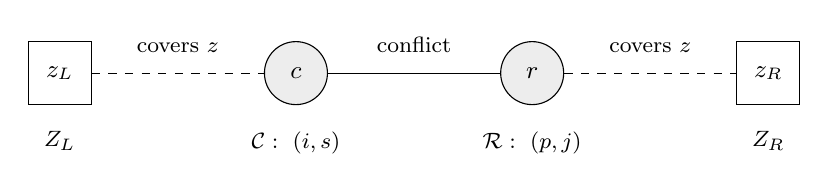
\begin{tikzpicture}[
  every node/.style={font=\small},
  original/.style={circle,draw,fill=black!7,minimum size=8mm,inner sep=1pt},
  copy/.style={rectangle,draw,minimum size=8mm,inner sep=3pt},
  edge label/.style={font=\footnotesize,above=4pt},
  family label/.style={font=\footnotesize,below=6pt}
]
 \node[copy] (zl) at (0,0) {$z_L$};
 \node[original] (c) at (3,0) {$c$};
 \node[original] (r) at (6,0) {$r$};
 \node[copy] (zr) at (9,0) {$z_R$};
 \draw[dashed] (zl) -- node[edge label] {covers $z$} (c);
 \draw (c) -- node[edge label] {conflict} (r);
 \draw[dashed] (r) -- node[edge label] {covers $z$} (zr);
 \node[family label] at (zl.south) {$Z_L$};
 \node[family label] at (c.south) {$\mathcal C:\ (i,s)$};
 \node[family label] at (r.south) {$\mathcal R:\ (p,j)$};
 \node[family label] at (zr.south) {$Z_R$};
\end{tikzpicture}

 \caption{A conflict between $r=(p,j)$ and $c=(i,s)$ forces this path,
 where $z=(i,j)\in Z$.  The copies $z_L$ and $z_R$ are distinct vertices.
 The vertices alternate between the two sides of the bipartition.
 Different conflicts can share vertices and edges; the full augmented
 graph need not be a disjoint union of such paths.}
 \label{fig:pruning}
\end{figure}

\step{Step 2: an initially conflict-free member is isolated in $\Gamma$.}
Let $(p,j)\in\mathcal R$ cover some $(i,j)\in Z$, so $p\to i$.
A conflict witnessing $(i,j)\in Z$ supplies a member $(i,s)\in\mathcal C$
with $s\to j$.  Then $(p,j)$ and $(i,s)$ conflict.  So a conflict-free
member of $\mathcal R$ has no edge of the first kind (by definition) and
none of the second kind.  The same argument with the sides exchanged
applies to $\mathcal C$.

\step{Step 3: a small vertex cover suffices.}
\emph{Claim.  If $K$ is a vertex cover of $\Gamma$ with
$\abs K\le\abs Z+\abs H$ that contains no isolated vertex, then
$\mathcal R'=\mathcal R\setminus K$ and $\mathcal C'=\mathcal C\setminus K$
satisfy the lemma.}

No conflict survives, since a conflict is an edge $r$---$c$ and one of its
ends is in $K$.  Conflict-free members are retained by Step~2.
For~\eqref{eq:pruning-bound}, let $q$ be the number of points of $Z$
covered by no surviving member.  Each of the other $\abs Z-q$ points $z$ is
covered by a surviving member, which is adjacent to $z_R$ or $z_L$.
The surviving member is not in $K$, so that copy of $z$ is in $K$.
Distinct points give distinct copies, so $K$ contains at least $\abs Z-q$
vertices of $Z_L\sqcup Z_R$, whence
\begin{equation}\label{eq:cover-charge}
 \abs{\mathcal R\setminus\mathcal R'}+\abs{\mathcal C\setminus\mathcal C'}
 =\abs{K\cap(\mathcal R\sqcup\mathcal C)}
 \leq \abs K-(\abs Z-q)\leq\abs H+q.
\end{equation}

\smallskip
It remains to produce such a cover.  We show that a maximum matching of
$\Gamma$ has at most $\abs Z+\abs H$ edges (Steps~4--10) and then construct
the cover from it (Step~11).

\step{Step 4: a special maximum matching.}
Among the maximum matchings of $\Gamma$ choose one, $\mathcal M$, with the
fewest edges of the first kind ($\mathcal R$---$\mathcal C$).  Let $k$ be
the number of these edges, and let $\alpha$ and $\beta$ be the sets of edges
of $\mathcal M$ of the second kind ($\mathcal R$---$Z_R$) and third kind
($Z_L$---$\mathcal C$).  Put
\[
 \ell=\abs\alpha,\qquad t=\abs\beta,
 \qquad\text{so}\qquad\abs{\mathcal M}=k+\ell+t.
\]
\emph{Claim.  $\alpha$ is a maximum matching of the subgraph of $\Gamma$ on
$\mathcal R\sqcup Z_R$, and $\beta$ is a maximum matching of the subgraph on
$Z_L\sqcup\mathcal C$.}

Suppose the $\mathcal R$---$Z_R$ subgraph has a matching $\alpha'$ with
$\abs{\alpha'}>\abs\alpha$.  The symmetric difference of $\alpha$ and
$\alpha'$ has maximum degree two, so some component is a path with more
edges of $\alpha'$ than of $\alpha$.  This is an $\alpha$-augmenting path:
its edges alternate, its two ends are $\alpha$-unmatched, and its internal
vertices are $\alpha$-matched.  Having odd length, it has one end
$r_0\in\mathcal R$ and one end $z_R\in Z_R$.  A vertex of $Z_R$ has
neighbors only in $\mathcal R$, so $z_R$ is unmatched in $\mathcal M$.  The
non-$\alpha$ edges of the path are $\mathcal R$---$Z_R$ edges not in
$\mathcal M$.
\begin{itemize}[nosep]
\item If $r_0$ is unmatched in $\mathcal M$, the path is
 $\mathcal M$-augmenting, and $\mathcal M$ was not maximum.
\item Otherwise $r_0$ is matched in $\mathcal M$ by an edge not in $\alpha$,
 hence of the first kind.  Remove that edge and augment along the path.
 The result is a matching of the same size as $\mathcal M$ with $k-1$
 edges of the first kind.
\end{itemize}
Both conclusions contradict the choice of $\mathcal M$.  The proof for
$\beta$ is the same with the sides exchanged.

Let $R_\alpha\subseteq\mathcal R$ and $C_\beta\subseteq\mathcal C$ be the
original members matched by $\alpha$ and by $\beta$.

\step{Step 5: four maps with $NL=AB$.}
For each pair $x\to y$ of the relation introduce two real parameters
$a_{xy}$ and $b_{xy}$; put $a_{xy}=b_{xy}=0$ when $x\not\to y$.  The values
are chosen in Step~7.  For any values, define four linear maps
\[
 \begin{array}{ccc}
 \R^{\mathcal R}&\xrightarrow{\ L\ }&\R^Z\\[3pt]
 {\scriptstyle B}\big\downarrow&&\big\downarrow{\scriptstyle N}\\[3pt]
 \R^H&\xrightarrow{\ A\ }&\R^{\mathcal C}
 \end{array}
\]
with entries
\begin{equation}\label{eq:pruning-maps}
 \begin{aligned}
 L_{(i,j),(p,j)}&=a_{pi},&
 N_{(i,s),(i,j)}&=b_{sj},\\
 B_{(p,s),(p,j)}&=b_{sj},&
 A_{(i,s),(p,s)}&=a_{pi},
 \end{aligned}
\end{equation}
where the row and column indices range over the indicated coordinate sets
and every entry not of a listed form is zero.  So an entry of $L$ or $A$ can
be nonzero only if row and column share their second coordinate, and an
entry of $N$ or $B$ only if they share their first coordinate.
In particular, $L_{z,r}\neq0$ implies that $r$ covers $z$, and
$N_{c,z}\neq0$ implies that $c$ covers $z$.  We claim
\begin{equation}\label{eq:pruning-commute}
 NL=AB.
\end{equation}
Fix a column $(p,j)\in\mathcal R$ and a row $(i,s)\in\mathcal C$.
In $(NL)_{(i,s),(p,j)}=\sum_{z\in Z}N_{(i,s),z}L_{z,(p,j)}$ a term can be
nonzero only if $z$ has first coordinate $i$ and second coordinate $j$.
So the sum is $b_{sj}a_{pi}$ if $(i,j)\in Z$ and $0$ otherwise.
Likewise $(AB)_{(i,s),(p,j)}$ is $a_{pi}b_{sj}$ if $(p,s)\in H$ and $0$
otherwise.  If $(p,j)$ and $(i,s)$ conflict, then $(i,j)\in Z$ and
$(p,s)\in H$, and both entries equal $a_{pi}b_{sj}$.  If they do not
conflict, then $p\not\to i$ or $s\not\to j$, so $a_{pi}b_{sj}=0$ and both
entries are $0$.

\step{Step 6: three rank conditions imply the matching bound.}
Suppose the parameters are such that
\begin{equation}\label{eq:three-conditions}
 \rank L=\ell,\qquad \rank N=t,\qquad \dim\ker A\geq k.
\end{equation}
Restricting $N$ to $\im L$ gives
\[
 \rank(NL)
 =\dim\im L-\dim(\im L\cap\ker N)
 \geq\ell-(\abs Z-t),
\]
since $\dim\ker N=\abs Z-t$.  By rank--nullity for $A$,
by $\im(AB)\subseteq\im A$, and by~\eqref{eq:pruning-commute},
\begin{align}
 \abs H
 &=\dim\ker A+\rank A
 \geq k+\rank(AB)= k+\rank(NL)
 \geq k+\ell+t-\abs Z.
 \label{eq:pruning-rank-bound}
\end{align}
That is, $\abs{\mathcal M}=k+\ell+t\le\abs Z+\abs H$.  Steps~7--10 produce
parameters satisfying~\eqref{eq:three-conditions}.

\step{Step 7: choice of the parameters.}
Regard the $a_{xy},b_{xy}$ ($x\to y$) as independent indeterminates.
The choice uses the correspondence between generic matrix rank and maximum
matching size~\cite[Section~5, Theorem~1]{Edmonds1967}; the parts needed
are proved here.  We list finitely many nonzero polynomials and then take a
real point at which none vanishes.

\emph{(a) $\rank L\le\ell$ and $\rank N\le t$ for every assignment.}
Let a square submatrix of $L$ with column set $\mathcal R_0\subseteq\mathcal R$
and row set $Z_0\subseteq Z$ have nonzero determinant.  Some term of the
Leibniz expansion is nonzero.  So there is a bijection
$\sigma:\mathcal R_0\to Z_0$ with $L_{\sigma(r),r}\neq0$ for all
$r\in\mathcal R_0$.  By Step~5 each $r$ covers $\sigma(r)$, so the edges
$r$---$\sigma(r)_R$ form a matching of size $\abs{\mathcal R_0}$ in the
$\mathcal R$---$Z_R$ subgraph.  By Step~4, $\abs{\mathcal R_0}\le\ell$.
The same argument for $N^{\mathsf T}$ (columns in $\mathcal C$, rows in $Z$)
with $\beta$ gives $\rank N=\rank N^{\mathsf T}\le t$.

\emph{(b) The minor of $L$ on the ends of $\alpha$ is a nonzero polynomial.}
Let $Z_\alpha\subseteq Z$ be the set of points whose right copies are matched
by $\alpha$.  Consider the square submatrix of $L$ with columns $R_\alpha$
and rows $Z_\alpha$.  An edge $r$---$z_R$ joins members with the same second
coordinate.  So for each $j\in X$, $\alpha$ matches the columns with second
coordinate $j$ to the rows with second coordinate $j$.  Entries between
different second coordinates vanish.  Hence, after ordering rows and columns
by $j$, the submatrix is block diagonal with square blocks, and its
determinant is $\pm$ the product of the block determinants.
In the block for $j$, the entry in row $(i,j)$ and column $(p,j)$ is the
indeterminate $a_{pi}$ if $p\to i$ and $0$ otherwise; distinct positions
carry distinct indeterminates.  In the Leibniz expansion of the block
determinant, each bijection all of whose positions are allowed contributes
$\pm$ the product of the indeterminates at its positions.  Different
bijections use different sets of positions, hence different monomials, so
nothing cancels.  The restriction of $\alpha$ is such a bijection.  So each
block determinant is a nonzero polynomial.  Indeterminates may recur in
different blocks, but a product of nonzero polynomials is nonzero.

\emph{(b$'$) The minor of $N^{\mathsf T}$ on the ends of $\beta$ is a nonzero
polynomial.}  This is the same argument with columns $C_\beta$ and rows the
points whose left copies are matched by $\beta$.  The blocks are indexed by
the common first coordinate $i$; the entry in row $(i,j)$ and column $(i,s)$
is $b_{sj}$.

\emph{(c) Support-rank minors.}
For every pair $p\to i$ of the relation, define
\[
 J_p=\{j:(p,j)\in\mathcal R\},\qquad
 S_i=\{s:(i,s)\in\mathcal C\},\qquad
 \Phi^{p,i}=(b_{sj})_{s\in S_i,\ j\in J_p},
\]
a matrix supported on
\[
 \Sigma^{p,i}=\{(s,j)\in S_i\times J_p:s\to j\},
\]
whose entries on $\Sigma^{p,i}$ are distinct indeterminates.
Let $\nu$ be the maximum rank of a real matrix supported on $\Sigma^{p,i}$,
attained by a real matrix $\Phi_0$, and choose a $\nu\times\nu$ submatrix of
$\Phi_0$ with nonzero determinant (the empty one if $\nu=0$).
The minor of $\Phi^{p,i}$ in the same rows and columns is a polynomial in the
$b$'s that is nonzero at the entries of $\Phi_0$.  So it is a nonzero
polynomial.  Take one such minor for each pair $p\to i$.

\emph{(d) The assignment.}
The product of the two polynomials of (b), (b$'$) and the finitely many of
(c) is a nonzero element of the polynomial ring in all the $a$'s and $b$'s.
A nonzero real polynomial is nonzero at some real point (induction on the
number of variables).  \emph{Fix such a point once and for all.}  At it:
\begin{enumerate}[label=\textup{(P\arabic*)},nosep,leftmargin=3em]
\item\label{P1} $\rank L=\ell$, and the columns $Le_\rho$
 ($\rho\in R_\alpha$) form a basis of $\im L$.  By (b) these $\ell$
 columns are independent, and by (a) the rank is at most $\ell$.
\item\label{P2} $\rank N=\rank N^{\mathsf T}=t$, and the columns
 $N^{\mathsf T}e_\gamma$ ($\gamma\in C_\beta$) form a basis of
 $\im N^{\mathsf T}$, by (b$'$) and (a).
\item\label{P3} For every pair $p\to i$, the real matrix $\Phi^{p,i}$ has
 maximum rank among all real matrices supported on $\Sigma^{p,i}$: its rank
 is $\ge\nu$ by (c) and $\le\nu$ by definition of $\nu$.
\end{enumerate}
The first two conditions of~\eqref{eq:three-conditions} now hold.

\step{Step 8: lifts.}
Let $(r,c)$ be one of the $k$ edges of $\mathcal M$ of the first kind,
$r\in\mathcal R$, $c\in\mathcal C$.  As $\mathcal M$ is a matching,
$r\notin R_\alpha$ and $c\notin C_\beta$.  By~\ref{P1},
$Le_r$ is a combination of the $Le_\rho$, and by~\ref{P2},
$N^{\mathsf T}e_c$ is a combination of the $N^{\mathsf T}e_\gamma$.
So there are reals $\lambda^r_\rho,\mu^c_\gamma$ with
\begin{equation}\label{eq:pruning-lifts}
 \begin{aligned}
 u^r&=e_r+\sum_{\rho\in R_\alpha}\lambda_\rho^r e_\rho
                 \in\ker L,\\
 v^c&=e_c+\sum_{\gamma\in C_\beta}\mu_\gamma^c e_\gamma
                 \in\ker N^{\mathsf T}.
 \end{aligned}
\end{equation}
If $r,r'$ are left ends of edges of the first kind, the coordinate of $u^r$
at $r'$ is $1$ if $r'=r$ and $0$ otherwise, because $r'\notin R_\alpha$.
Also the coordinate of $v^c$ at $c$ is $1$.

\step{Step 9: the kernel restriction.}
For $u\in\R^{\mathcal R}$ and $v\in\R^{\mathcal C}$ write $u_{pj}$ and
$v_{is}$ for the coordinates at $(p,j)\in\mathcal R$ and
$(i,s)\in\mathcal C$.  \emph{Claim: at the fixed assignment,}
\begin{equation}\label{eq:conflict-kernel}
 u_{pj}v_{is}=0
 \quad\text{for every conflict }((p,j),(i,s)),
 \quad\text{every }u\in\ker B,\quad\text{every }v\in\ker N^{\mathsf T}.
\end{equation}
Fix such a conflict, $u$ and $v$.  Then $p\to i$, $j\in J_p$, $s\in S_i$
and $s\to j$, so $(s,j)\in\Sigma^{p,i}$.  Put
\[
 \mathbf x=(u_{pj'})_{j'\in J_p}\in\R^{J_p},\qquad
 \mathbf y=(v_{is'})_{s'\in S_i}\in\R^{S_i}.
\]

\emph{(a) $\mathbf x\in\ker\Phi^{p,i}$.}  Fix a row $s'\in S_i$; we must show
\begin{equation}\label{eq:pruning-row-equation}
 \sum_{j'\in J_p}b_{s'j'}u_{pj'}=0.
\end{equation}
If $s'\not\to j'$ for all $j'\in J_p$, every coefficient is zero.
Otherwise pick $j'\in J_p$ with $s'\to j'$.  Then $(p,j')\in\mathcal R$ and
$(i,s')\in\mathcal C$ conflict (using $p\to i$), so $(p,s')\in H$.
By~\eqref{eq:pruning-maps}, row $(p,s')$ of $B$ has entry $b_{s'j'}$ in each
column $(p,j')$, $j'\in J_p$, and zero in every other column.  So the left
side of~\eqref{eq:pruning-row-equation} is the $(p,s')$-coordinate of $Bu$,
which is $0$.

\emph{(b) $\mathbf y\in\ker(\Phi^{p,i})^{\mathsf T}$.}  Fix a column
$j'\in J_p$; we must show
\begin{equation}\label{eq:pruning-column-equation}
 \sum_{s'\in S_i}b_{s'j'}v_{is'}=0.
\end{equation}
If $s'\not\to j'$ for all $s'\in S_i$, every coefficient is zero.
Otherwise pick $s'\in S_i$ with $s'\to j'$.  The resulting conflict of
$(p,j')$ and $(i,s')$ gives $(i,j')\in Z$.  By~\eqref{eq:pruning-maps},
column $(i,j')$ of $N$ has entry $b_{s'j'}$ in each row $(i,s')$,
$s'\in S_i$, and zero elsewhere.  So the left side
of~\eqref{eq:pruning-column-equation} is the $(i,j')$-coordinate of
$N^{\mathsf T}v$, which is $0$.

\emph{(c)} By~\ref{P3}, Lemma~\ref{lem:kernel-support} applies to
$\Phi^{p,i}$ with support $\Sigma^{p,i}$, and gives
$\mathbf x_j\mathbf y_s=u_{pj}v_{is}=0$.
The perturbation inside the proof of that lemma concerns only
$\Phi^{p,i}$ as an abstract matrix supported on $\Sigma^{p,i}$; it does not
change our fixed assignment.

\step{Step 10: $\dim\ker A\ge k$.}
Let $(r,c)$ be an edge of $\mathcal M$ of the first kind; it is a conflict.
Apply~\eqref{eq:conflict-kernel} with $v=v^c$, whose coordinate at $c$
is~$1$: every $u\in\ker B$ has coordinate $0$ at $r$.
Now let $r$ range over the $k$ left ends of such edges and suppose
\[
 \sum_r\theta_r Bu^r=0 .
\]
Then $u=\sum_r\theta_r u^r\in\ker B$, and by Step~8 its coordinate at each
such $r$ is $\theta_r$.  These coordinates vanish, so all $\theta_r=0$.
So the $k$ vectors $Bu^r$ are linearly independent.  They lie in $\ker A$,
since
\[
 A(Bu^r)=NLu^r=0
\]
by~\eqref{eq:pruning-commute} and $u^r\in\ker L$.  Thus $\dim\ker A\geq k$.
All of~\eqref{eq:three-conditions} holds, and Step~6 gives
$\abs{\mathcal M}=k+\ell+t\leq\abs Z+\abs H$.

\step{Step 11: from the matching bound to a cover.}
This is the matching-to-cover argument in K\H{o}nig's
theorem~\cite{konig1931}, included for completeness.  Starting at all
$\mathcal M$-unmatched vertices of $\mathcal V_L$, follow edges outside
$\mathcal M$ from left to right and edges in $\mathcal M$ from right to left.
Let $W_L,W_R$ be the sets of reached vertices on the two sides, and put
\[
 K=(\mathcal V_L\setminus W_L)\cup W_R .
\]
\begin{enumerate}[label=\textup{(\alph*)},nosep]
\item No unmatched right vertex is reached: an alternating path to one
 would augment the maximum matching $\mathcal M$.
\item The two ends of a matched edge are both reached or both unreached.
 A reached right end leads to its mate.  A matched left vertex is not a
 starting vertex, and can be entered only along its matching edge, i.e.\
 from its mate.
\item $K$ covers every edge.  An uncovered edge would join a reached left
 vertex to an unreached right vertex.  It is not outside $\mathcal M$ (it
 would have been traversed) and not in $\mathcal M$ (by (b)).
\item $\abs K=\abs{\mathcal M}$.  Every vertex of $K$ is matched:
 unmatched left vertices are in $W_L$, and reached right vertices are
 matched by (a).  By (b), $K$ contains exactly one end of each matched edge.
\item $K$ contains no isolated vertex, since isolated vertices are
 unmatched and vertices of $K$ are matched.
\end{enumerate}
Hence $\abs K=\abs{\mathcal M}\leq\abs Z+\abs H$, and Step~3 applied to this
$K$ proves the lemma.
\end{proof}

\section{The extremal contradiction}\label{sec:incompatibility}

This section is Part C: Lemma~\ref{lem:pruning} is used to rule out the graph
supplied by Proposition~\ref{prop:counterexample-reduction}.

\begin{proposition}\label{prop:no-concavity}
There is no nonempty finite oriented graph $G$ in which every vertex has an
in-neighbor and whose one-step image operator
\[
 F(U)=\{y\in V(G):x\to y\text{ for some }x\in U\}
\]
satisfies
\begin{equation}\label{eq:impossible-concavity}
 \abs{U}+\abs{F^2(U)}<2\abs{F(U)}
 \qquad(\varnothing\ne U\subsetneq V(G)),
\end{equation}
where $F^2=F\circ F$.
\end{proposition}

\emph{Plan of the proof.}  Assume $G$ exists.  Choose a compatible pair
$(P,Q)$ of families of ordered pairs, containing the diagonal, that
maximizes $M+d$ (Steps~1--2).  Inequality~\eqref{eq:impossible-concavity},
applied columnwise to $P$ and rowwise to $Q$, makes the complements
$\mathcal R,\mathcal C$ of $F_2^2Q,F_1^2P$ large (Steps~3--4).  Prune them by
Lemma~\ref{lem:pruning}, after checking that the diagonal survives
(Steps~5--6) and that $\abs H\le d$ (Step~7).  The result beats the maximum
(Step~8).

\begin{proof}
Suppose that such a graph exists, and put $X=V(G)$; here $F=F_G$.

\step{Step 1: coordinate images and compatibility.}
For $\mathcal S\subseteq X\times X$, define
\[
 \begin{aligned}
 F_1\mathcal S&=\{(i,j): (p,j)\in \mathcal S\text{ and }p\to i
                     \text{ for some }p\in X\},\\
 F_2\mathcal S&=\{(i,j): (i,s)\in \mathcal S\text{ and }s\to j
                     \text{ for some }s\in X\}.
 \end{aligned}
\]
Write $F_1^2=F_1\circ F_1$, $F_2^2=F_2\circ F_2$, and
$\Delta=\{(v,v):v\in X\}$.  Two facts follow from the definitions.
\begin{enumerate}[label=\textup{(\alph*)},nosep]
\item \emph{Fibres.}  For the column $\mathcal S_j=\{p:(p,j)\in\mathcal S\}$,
 the $j$-th column of $F_1\mathcal S$ is $F(\mathcal S_j)$ and that of
 $F_1^2\mathcal S$ is $F^2(\mathcal S_j)$.  Symmetrically, the $i$-th row of
 $F_2\mathcal S$ (resp.\ $F_2^2\mathcal S$) is $F$ (resp.\ $F^2$) of the
 $i$-th row $\{s:(i,s)\in\mathcal S\}$ of $\mathcal S$.
\item \emph{Compatibility is absence of conflicts.}  Call
 $P,Q\subseteq X\times X$ \emph{compatible} if
 $F_1P\cap F_2Q=\varnothing$.  A point $(i,j)$ lies in $F_1P\cap F_2Q$
 exactly when there are $(p,j)\in P$ and $(i,s)\in Q$ with $p\to i$ and
 $s\to j$.  So $P,Q$ are compatible if and only if no member of $P$
 conflicts with a member of $Q$, in the sense of Lemma~\ref{lem:pruning}
 with $\mathcal R=P$, $\mathcal C=Q$.  In that lemma's language, the points
 covered by members of $P$ are exactly those of $F_1P$, and the points
 covered by members of $Q$ are exactly those of $F_2Q$.
\end{enumerate}

\step{Step 2: the extremal choice.}
The pair $P=Q=\Delta$ is compatible: $(i,j)\in F_1\Delta$ means $j\to i$,
and $(i,j)\in F_2\Delta$ means $i\to j$; both together contradict
orientation.  Since $X$ is finite we may choose, among all compatible pairs
with $\Delta\subseteq P\cap Q$, one maximizing $M+d$, where
\[
 M=\abs{P}+\abs{Q},\qquad
 d=\abs{X}^2-\abs{F_1P}-\abs{F_2Q}.
\]
By compatibility, $d$ is the number of points outside $F_1P\cup F_2Q$.

\step{Step 3: columns of $P$ and rows of $Q$ are nonempty and proper.}
The column $P_j=\{p:(p,j)\in P\}$ contains $j$.  Suppose $P_j=X$.
Positive indegrees give $F(X)=X$ by~\ref{F3}, so by Step~1(a),
$X\times\{j\}\subseteq F_1P$.  Choose an in-neighbor $w$ of $j$.  Then
$(w,j)\in F_2\Delta\subseteq F_2Q$ (from $(w,w)\in\Delta$ and $w\to j$),
and also $(w,j)\in F_1P$, contradicting compatibility.
Likewise the row $Q_i=\{s:(i,s)\in Q\}$ contains $i$.  If $Q_i=X$, then
$\{i\}\times X\subseteq F_2Q$.  Choosing $w\to i$ gives
$(i,w)\in F_1\Delta\subseteq F_1P$, again a contradiction.

So~\eqref{eq:impossible-concavity} applies to each $P_j$ and each $Q_i$.
Summing over $j\in X$ and over $i\in X$ (nonempty index sets, each
inequality strict) and using Step~1(a),
\begin{equation}\label{eq:strict-fiber-sums}
 \abs{P}+\abs{F_1^2P}<2\abs{F_1P},\qquad
 \abs{Q}+\abs{F_2^2Q}<2\abs{F_2Q}.
\end{equation}

\step{Step 4: the prospective families.}
Define
\[
 \mathcal R=(X\times X)\setminus F_2^2Q,
 \qquad
 \mathcal C=(X\times X)\setminus F_1^2P.
\]
By~\eqref{eq:strict-fiber-sums},
\begin{equation}\label{eq:complement-gain}
 \begin{aligned}
 \abs{\mathcal R}+\abs{\mathcal C}
 &=2\abs{X}^2-\abs{F_2^2Q}-\abs{F_1^2P}\\
 &>2\abs{X}^2+\abs Q-2\abs{F_2Q}+\abs P-2\abs{F_1P}
 =M+2d.
 \end{aligned}
\end{equation}
These families need not be compatible.

\step{Step 5: both families contain $\Delta$.}
If $(v,v)\in F_2^2Q$, there is $s\to v$ with $(v,s)\in F_2Q$.
But $(s,s)\in P$ and $s\to v$ give $(v,s)\in F_1P$, contradicting
compatibility of $P,Q$.  So $\Delta\subseteq\mathcal R$.
If $(v,v)\in F_1^2P$, there is $p\to v$ with $(p,v)\in F_1P$.
But $(p,p)\in Q$ and $p\to v$ give $(p,v)\in F_2Q$, the same contradiction.
So $\Delta\subseteq\mathcal C$.

\step{Step 6: diagonal members are conflict-free in
$(\mathcal R,\mathcal C)$.}
Suppose the left member $(v,v)\in\mathcal R$ conflicts with some
$(i,s)\in\mathcal C$, i.e.\ $v\to i$ and $s\to v$.  From $(s,s)\in P$ and
$s\to v$ we get $(v,s)\in F_1P$, and then $v\to i$ gives
$(i,s)\in F_1^2P$, contrary to $(i,s)\in\mathcal C$.
Suppose some $(p,j)\in\mathcal R$ conflicts with the right member
$(v,v)\in\mathcal C$, i.e.\ $p\to v$ and $v\to j$.  From $(p,p)\in Q$ and
$p\to v$ we get $(p,v)\in F_2Q$, and then $v\to j$ gives
$(p,j)\in F_2^2Q$, contrary to $(p,j)\in\mathcal R$.

\step{Step 7: $\abs H\le d$.}
Let $H,Z\subseteq X\times X$ be the sets attached to
$\mathcal R,\mathcal C$ in Lemma~\ref{lem:pruning}: each conflict
\[
 (p,j)\in\mathcal R,\quad (i,s)\in\mathcal C,\quad
 p\to i,\quad s\to j
\]
contributes $(p,s)$ to $H$ and $(i,j)$ to $Z$.  We claim
\begin{equation}\label{eq:old-uncovered-bound}
 H\subseteq (X\times X)\setminus(F_1P\cup F_2Q),
 \qquad\text{and hence}\qquad \abs{H}\le d.
\end{equation}
Fix such a conflict.  If $(p,s)\in F_1P$, then $p\to i$ gives
$(i,s)\in F_1^2P$, contrary to $(i,s)\in\mathcal C$.
If $(p,s)\in F_2Q$, then $s\to j$ gives $(p,j)\in F_2^2Q$, contrary to
$(p,j)\in\mathcal R$.  The bound $\abs H\le d$ follows from Step~2.

\step{Step 8: pruning and the count.}
Apply Lemma~\ref{lem:pruning} to $X$, the arc relation of $G$, and
$\mathcal R,\mathcal C$.  It gives conflict-free
$P'\subseteq\mathcal R$ and $Q'\subseteq\mathcal C$ retaining all
conflict-free members.  By Steps~5--6, $\Delta\subseteq P'\cap Q'$.
By Step~1(b), $F_1P'\cap F_2Q'=\varnothing$.  So $(P',Q')$ is one of the
pairs over which $M+d$ was maximized.  Set
\[
 d'=\abs{X}^2-\abs{F_1P'}-\abs{F_2Q'},
\]
the number of points outside $F_1P'\cup F_2Q'$.  By Step~1(b), these are
exactly the points covered by no member of $P'\cup Q'$.  So at most $d'$
points of $Z$ are uncovered after pruning.
By~\eqref{eq:pruning-bound} and~\eqref{eq:old-uncovered-bound},
\[
 \abs{\mathcal R\setminus P'}+\abs{\mathcal C\setminus Q'}\le\abs H+d'
 \le d+d'.
\]
Using~\eqref{eq:complement-gain},
\[
 \begin{aligned}
 \abs{P'}+\abs{Q'}+d'
 &\ge \abs{\mathcal R}+\abs{\mathcal C}-(d+d')+d'\\
 &>M+2d-(d+d')+d'=M+d.
 \end{aligned}
\]
This contradicts the maximality of $M+d$ and proves the proposition.
\end{proof}

\begin{proof}[Proof of Theorem~\ref{thm:main}]
If the theorem were false, Proposition~\ref{prop:counterexample-reduction}
would produce a nonempty finite oriented graph with positive indegrees
satisfying~\eqref{eq:impossible-concavity} for every nonempty proper vertex
set (\eqref{eq:strict-subset-growth} and~\eqref{eq:impossible-concavity} are
the same condition).  Proposition~\ref{prop:no-concavity} rules out such a
graph.
\end{proof}

\section{Weighted consequences}\label{sec:weighted-consequences}

The following corollary applies Theorem~\ref{thm:main} through Seacrest's
established equivalences of the corresponding assertions over all nonempty
finite oriented graphs~\cite{Seacrest2015}.  The equivalences themselves are
not new here.  The proof uses two results from~\cite{Seacrest2015}, stated
here as the source describes them; I did not have the reference at hand.
\begin{itemize}[nosep]
\item \emph{Seacrest's Proposition~2.}  The assertion ``statement
 \textup{(iii)} below holds for every nonempty finite oriented graph and
 every arc weighting'' (his arc-weighted Conjecture~4) is equivalent to the
 assertion ``the conclusion of Theorem~\ref{thm:main} holds for every
 nonempty finite oriented graph''.
\item \emph{The Farkas alternative used in Seacrest's Theorem~1.}  For a real
 matrix $\mathsf M$, either there is a nonzero vector $\eta\ge0$ with
 $\mathsf M\eta\ge0$, or there is a vector $\xi\ge0$ with
 $\mathsf M^{\mathsf T}\xi<0$ in every coordinate.
\end{itemize}

\begin{corollary}[Weighted second-neighborhood forms]\label{cor:weighted-forms}
Let \(D\) be a nonempty finite oriented graph, and write \(A(D)\) for its
arc set.  For a vertex weighting \(\eta:V(D)\to[0,\infty)\), write
\(\eta(S)=\sum_{x\in S}\eta(x)\).  Then the following hold.
\begin{enumerate}[label=\textup{(\roman*)}]
\item For every vertex weighting \(\eta:V(D)\to[0,\infty)\), there is a
vertex \(v\in V(D)\) such that
\[
 \eta(N_1^+(v))\leq\eta(N_2^+(v)).
\]

\item There is a vertex weighting \(\eta:V(D)\to[0,\infty)\) with
\(\sum_{x\in V(D)}\eta(x)=1\) such that
\[
 \eta(N_1^+(v))\leq\eta(N_2^+(v))\qquad\text{for every }v\in V(D).
\]
The entries of this weighting need not all be positive.

\item For every arc weighting \(\omega:A(D)\to[0,\infty)\), extend the
notation by setting \(\omega(vs)=0\) when \(vs\notin A(D)\).  For
\(v,s\in V(D)\), put
\[
 \kappa_v^\omega(s)=\max\Bigl(\{0\}\cup
 \{\omega(us)-\omega(vs):u\in V(D),\ v\to u\to s\}\Bigr).
\]
Then there is a vertex \(v\in V(D)\) such that
\[
 \sum_{s\in V(D)}\kappa_v^\omega(s)
 \geq \sum_{u\in N_1^+(v)}\omega(vu).
\]
The maximum is zero if there is no indicated two-step path.  Such paths
are determined by the arcs of \(D\), so an arc of weight zero is still
present and is not treated as a missing arc.
\end{enumerate}
\end{corollary}

\begin{proof}
\emph{\textup{(iii)}.}  Theorem~\ref{thm:main} is the unweighted assertion
for all graphs, so Seacrest's Proposition~2 gives \textup{(iii)}.

\emph{\textup{(i)} from \textup{(iii)}.}  Set $\omega(us)=\eta(s)$ on every
arc $u\to s$, and fix $v$.  We claim
\[
 \kappa_v^\omega(s)=
 \begin{cases}
  \eta(s),&s\in N_2^+(v),\\
  0,&s\notin N_2^+(v).
 \end{cases}
\]
If $v\to s$, every eligible difference is
$\omega(us)-\omega(vs)=\eta(s)-\eta(s)=0$.  If $s\in N_2^+(v)$, then
$\omega(vs)=0$, there is at least one path $v\to u\to s$, and every
eligible difference is $\eta(s)\ge0$.  In the remaining cases ($s=v$, or
$s$ not reachable in two steps) there is no path $v\to u\to s$: for $s=v$
this is orientation.  Hence the two sides of \textup{(iii)} are
$\eta(N_2^+(v))$ and $\sum_{u\in N_1^+(v)}\eta(u)=\eta(N_1^+(v))$.
This is the specialization noted immediately after Seacrest's
Proposition~2.

\emph{\textup{(ii)}.}  Let $\mathsf M_D$ be the $V(D)\times V(D)$ matrix
with entry $1$ at $(v,s)$ when $s\in N_2^+(v)$, entry $-1$ when
$s\in N_1^+(v)$, and zero otherwise.  Then $(\mathsf M_D\eta)_v
=\eta(N_2^+(v))-\eta(N_1^+(v))$.  Let $\overleftarrow D$ be $D$ with all
arcs reversed; it is again a nonempty finite oriented graph.
Reversal transposes the matrix,
$\mathsf M_{\overleftarrow D}=\mathsf M_D^{\mathsf T}$: the conditions
``$v\to s$'' and ``$v\ne s$, $v\not\to s$, and $v\to u\to s$ for some $u$''
in $\overleftarrow D$ are the same conditions in $D$ with $v$ and $s$
exchanged.
By the Farkas alternative, either there is a nonzero $\eta\ge0$ with
$\mathsf M_D\eta\ge0$, or there is $\xi\ge0$ with
$\mathsf M_D^{\mathsf T}\xi=\mathsf M_{\overleftarrow D}\xi<0$ at every
coordinate.  The latter says $\xi(N_2^+(v))<\xi(N_1^+(v))$ for every vertex
$v$ of $\overleftarrow D$, contradicting \textup{(i)} for
$\overleftarrow D$.  So the former holds; dividing $\eta$ by its total
weight gives \textup{(ii)}.
\end{proof}

\section{Directed-cycle consequences}\label{sec:directed-cycle-consequences}

In an oriented graph with no directed triangle, every exact second
out-neighbor is a non-neighbor.  Combining this observation with
Theorem~\ref{thm:main} gives degree and order bounds.
The first assertion below is the oriented-graph form of Thomass\'e's
non-neighbor statement recorded by
Sullivan~\cite[Conjecture~6.12]{Sullivan2006}.
The consequence using both minimum indegree and minimum outdegree is also
noted in \cite[Section~3]{Sullivan2006}.  The regular case gives the
girth-four lower bound in the Behzad--Chartrand--Wall minimum-order
conjecture~\cite{BehzadChartrandWall1970}, also recorded by
Sullivan~\cite[Section~4]{Sullivan2006}.

\begin{corollary}[Non-neighbors and directed cycles]\label{cor:directed-cycle-consequences}
Let \(D\) be a nonempty finite oriented graph of order \(n\).  For
\(v\in V(D)\), write
\[
 N_1^-(v)=\{u:u\to v\},\qquad
 d^\pm(v)=\abs{N_1^\pm(v)},\qquad
 \delta^\pm(D)=\min_{x\in V(D)}d^\pm(x).
\]
Define the non-neighbors of \(v\), excluding \(v\) itself, by
\[
 N^0(v)=V(D)\setminus
 \bigl(\{v\}\cup N_1^+(v)\cup N_1^-(v)\bigr).
\]
Then the following hold.
\begin{enumerate}[label=\textup{(\roman*)}]
\item If \(D\) has no directed \(3\)-cycle, then some vertex \(v\) satisfies
\[
 d^+(v)\leq\abs{N^0(v)},\qquad
 n-1\geq 2d^+(v)+d^-(v).
\]
\item If \(\delta^+(D)\geq n/3\) and \(\delta^-(D)\geq n/3\), then \(D\)
contains a directed \(3\)-cycle.
\item If \(r\geq1\) is an integer, \(d^+(v)=d^-(v)=r\) for every vertex,
and \(D\) has directed girth exactly four, then \(n\geq3r+1\).
\end{enumerate}
Here directed girth is the length of a shortest directed cycle.
\end{corollary}

\begin{proof}
\emph{\textup{(i)}.}  Suppose that \(D\) has no directed \(3\)-cycle.
Let \(w\in N_2^+(v)\) and choose a path \(v\to u\to w\).  By definition
\(w\ne v\) and \(w\notin N_1^+(v)\).  If \(w\in N_1^-(v)\), the arc
\(w\to v\) would close the directed \(3\)-cycle $v\to u\to w\to v$.  Thus
\(N_2^+(v)\subseteq N^0(v)\) for every \(v\).  Theorem~\ref{thm:main}
gives a vertex with
\[
 d^+(v)\leq\abs{N_2^+(v)}\leq\abs{N^0(v)}.
\]
Since \(D\) is oriented, $N_1^+(v)$ and $N_1^-(v)$ are disjoint, so
$V(D)\setminus\{v\}$ is the disjoint union of $N_1^+(v)$, $N_1^-(v)$ and
$N^0(v)$.  Hence
\[
 n-1=d^+(v)+d^-(v)+\abs{N^0(v)}
 \geq 2d^+(v)+d^-(v).
\]

\emph{\textup{(ii)}.}  If $D$ had no directed \(3\)-cycle, \textup{(i)}
would give
\[
 n-1\geq2d^+(v)+d^-(v)\geq2\delta^+(D)+\delta^-(D)\geq n,
\]
a contradiction.  (The hypotheses are real inequalities
$\delta^\pm(D)\ge n/3$, so the endpoint case $3\mid n$,
$\delta^\pm(D)=n/3$ is included.)

\emph{\textup{(iii)}.}  Directed girth four excludes directed
\(3\)-cycles, and in the regular case the count in \textup{(i)} becomes
\(n-1\geq3r\).
\end{proof}

\section{Verification checklist}\label{sec:checklist}

The following steps carry the proof; a sceptical reader should check them
first.

\begin{enumerate}[leftmargin=2em]
\item \textbf{The flagged sentence.}
 Lemma~\ref{lem:subset-deficit}, Step~1: the source's choice of a
 component with no \emph{incoming} arc does not justify strong
 connectivity as written.  Check that the argument works for a component
 with no \emph{outgoing} arc, and that nothing else depends on the choice
 (strong connectivity is used only in Steps~2 and~3 of that proof).
\item \textbf{Arc-deletion bookkeeping.}
 Lemma~\ref{lem:subset-deficit}, Steps~4c--4g: the
 inclusion~\eqref{eq:deleted-path-endpoints}, the inclusions ``gains
 $\subseteq Y\cap F(T)$'' and ``$C\subseteq$ losses'', and the exact
 identity $g(T\cup Y)-g(T)=\abs C-\abs{Y\cap F(T)}$.  The strictness
 in~\eqref{eq:subset-deficit} comes only from $d_2<d_1$.
\item \textbf{Blow-up arithmetic.}
 Lemma~\ref{lem:blowup}, Steps~4--7: the exact formula for
 $\abs{F_G(U)}$, the block-by-block bound for $\abs{F_G^2(U)}$, and the
 final estimate $\le -m+n<0$, which is where $m>n$ is used.  Also Step~8
 for the case $S=V(D)$, where~\eqref{eq:subset-deficit} is unavailable.
\item \textbf{The charging argument.}
 Lemma~\ref{lem:pruning}, Steps~2--3: conflict-free members are isolated
 in $\Gamma$, and a cover $K$ with $\abs K\le\abs Z+\abs H$
 gives~\eqref{eq:cover-charge}.  This is where the ``uncovered after
 pruning'' term arises.
\item \textbf{The commuting square and the rank chain.}
 Lemma~\ref{lem:pruning}, Steps~5--6: the identity $NL=AB$
 of~\eqref{eq:pruning-commute}, and the
 chain~\eqref{eq:pruning-rank-bound} from the three
 conditions~\eqref{eq:three-conditions}.
\item \textbf{One assignment serving all rank conditions.}
 Lemma~\ref{lem:pruning}, Step~7 (each listed minor is a nonzero
 polynomial, so one real point works for all), then
 Lemma~\ref{lem:kernel-support} and Step~9 (the vectors
 $\mathbf x,\mathbf y$ really lie in the kernels of $\Phi^{p,i}$ and its
 transpose, including rows and columns with no allowed entry), and
 Step~10 ($\dim\ker A\ge k$).  Step~4 (maximality of $\alpha$ and
 $\beta$) is what makes $\rank L\le\ell$ and $\rank N\le t$.
\item \textbf{The extremal count.}
 Proposition~\ref{prop:no-concavity}: Step~3 (columns and rows are proper;
 this uses positive indegree), Step~4 ($>M+2d$), Steps~5--6 (the diagonal
 survives pruning), Step~7 ($\abs H\le d$), and the final display of
 Step~8.
\item \textbf{External inputs.}  Theorem~\ref{thm:main} uses no result
 beyond those proved above (the citations to~\cite{Edmonds1967}
 and~\cite{konig1931} are for attribution; the needed arguments are
 written out).  Corollary~\ref{cor:weighted-forms} relies on the two
 statements quoted from~\cite{Seacrest2015} at the start of
 Section~\ref{sec:weighted-consequences}.
\end{enumerate}

\bibliographystyle{plain}
\bibliography{references}
\end{document}
